
%%%%%%%%%%%%%%%%%%%%%%% file typeinst.tex %%%%%%%%%%%%%%%%%%%%%%%%%
%
% This is the LaTeX source for the instructions to authors using
% the LaTeX document class 'llncs.cls' for contributions to
% the Lecture Notes in Computer Sciences series.
% http://www.springer.com/lncs       Springer Heidelberg 2006/05/04
%
% It may be used as a template for your own input - copy it
% to a new file with a new name and use it as the basis
% for your article.
%
% NB: the document class 'llncs' has its own and detailed documentation, see
% ftp://ftp.springer.de/data/pubftp/pub/tex/latex/llncs/latex2e/llncsdoc.pdf
%
%%%%%%%%%%%%%%%%%%%%%%%%%%%%%%%%%%%%%%%%%%%%%%%%%%%%%%%%%%%%%%%%%%%


\documentclass[runningheads,a4paper]{llncs}

\usepackage{amssymb}
\setcounter{tocdepth}{3}
\usepackage{graphicx}
\usepackage{times,amsmath,epsfig}
\usepackage[linesnumbered,ruled,vlined]{algorithm2e}
\usepackage{subfigure}

\usepackage{url}
%\urldef{\mailsa}\path|{alfred.hofmann, ursula.barth, ingrid.haas, frank.holzwarth,|
%\urldef{\mailsb}\path|anna.kramer, leonie.kunz, christine.reiss, nicole.sator,|
%\urldef{\mailsc}\path|erika.siebert-cole, peter.strasser, lncs}@springer.com|
%\newcommand{\keywords}[1]{\par\addvspace\baselineskip
%\noindent\keywordname\enspace\ignorespaces#1}


\begin{document}

\mainmatter  % start of an individual contribution

\pagestyle{empty}

% first the title is needed
\title{Mining Probabilistic High Utility Itemsets in Uncertain Databases}

\author{
Yuqing Lan
        \and 
Shengwei Yi
        \and 
Dan Yu
        \and
Jie Liang
}

\institute{School of Computer Science and Engineering, Beihang University, China\\
\email{\{lanyuqing, yishengwei, yudan, liangjie\}@buaa.edu.cn}}


\maketitle


\begin{abstract}
Recently, with the growing popularity of Internet of Things (IoT) and pervasive computing, a large amount
of uncertain data, i.e. RFID data, sensor data, real-time monitering data, etc., has been collected. As one of the most fundamental issues of uncertain data mining, the problem of mining uncertain frequent itemsets has attracted much attention in the database and data mining communities. Although some efficient approaches of mining uncertain frequent itemsets have been proposed, most of them only consider each item in one transaction as a random variable following the binary distribution and ignore the unit profits of items in the real scenarios. In this paper, we focus on the problem of \textit{\underline{m}ining \underline{p}robabilistic \underline{h}igh \underline{u}tility itemsets in uncertain databases} (MPHU), in which each item has an unit profit and likely appears multiple times in one transaction. In order to solve the \textit{MPHU} problem, we propose a novel mining framework, called \textit{UUIM}, which not only includes an efficient mining algorithm but also contains an effective pruning technique. Extensive experiments on both real and synthetic datasets verify the effectiveness and efficiency of proposed solutions.
\end{abstract}


\section{Introduction}

Data mining approach aims to derive the useful information from the massive data. In many application scenarios, what people generally concerned about are high frequent item sets, because this kind of item sets tend to have greater influence and improvements based on them are often the most effective. It can be said that people already have some effective solution of the uncertain transaction data set mining problem. But can they completely solve the problem of uncertain transaction data set? Let's see an example:

As we all know, from the beginning of human emergence, disease is the main reason which affect human health. According to WHO, in 2011, the number of some infectious disease cases in worldwide are more than 30 million\cite{bib1}. If we statistic and summary the incidence of them, we can get a big data set where data mining approach can be useful. Table 1 shows the incidence of cases, it's a typical uncertain transaction data set which holds 5 transactions.

\begin{table}[htbp]
\caption{Statistic of patient incidences}
\centering
{
\begin{tabular}{|c|c|c|c|c|c|c|c|}\hline
{Patient}{Incidence} & Apocleisis(A) & Drowsiness(B) & Fever(C) & Cold(D) & Gastritis(E) & Appendicitis(F) & Lung cancer(G) \\ \hline
1. Zhao & 0.2 & 0.3 & 0.05 & 0.02 & 0 & 0 & 0 \\ \hline
2. Qian & 0 & 0.2 & 0.045 & 0.015 & 0 & 0 & 0 \\ \hline
3. Sun & 0.1 & 0.3 & 0.055 & 0.01 & 0.005 & 0 & 0 \\ \hline
4. Li & 0.2 & 0.2 & 0.06 & 0 & 0.004 & 0.002 & 0 \\ \hline
5. Zhou & 0.3 & 0.4 & 0.04 & 0.015 & 0 & 0 & 0.001 \\ \hline
\end{tabular}
\vspace{-0.3cm}
}
\label{sopi}
\end{table}


The decimal number in table represent the incidence of patients . For example, Zhao shows the incidence of apocleisis in two of ten days on average. The incidences of each patients in table is a transaction, each incidence is an item. If we use the traditional data mining approach we will obviously get frequent itemset like {A}, {B}, {A, B}. But these are not what we want, the reason is that even if they appear frequent, their impact on human health is not very high, whereas diseases which do great harm to human such as gastritis and lung cancer are not found out. So the answer of the previous question is, frequent data mining approaches in uncertain environment cannot solve the problem entirely.

What should we do? We can get inspiration from the existing work of certain data mining and give the corresponding profit of each item based on it's importance. For example, table 2 shows the profit of each incidence in table 4 based on their harm to human beings. Hence, we can combine frequency and profit to find out useful information.

\begin{table}[htbp]
\caption{the profit of each incidence}
\centering
{
\begin{tabular}{|c|c|c|c|c|c|c|c|}\hline
Incidence & Apocleisis(A) & Drowsiness(B) & Fever(C) & Cold(D) & Gastritis(E) & Appendicitis(F) & Lung cancer(G) \\ \hline
profit & 1 & 1 & 5 & 10 & 100 & 500 & 1000 \\ \hline
\end{tabular}
}
\label{tpoei}
\end{table}

Therefore, in this paper, we address the above challenges and make the following contributions:

\begin{itemize}
  \item To the best of our knowledge, this is the first work to formulate the problem of \underline{m}ining \underline{p}robabilistic \underline{h}igh \underline{u}tility itemsets in uncertain databases (MPHU). 
  \item Due to the challenges from utility constraints, we propose a novel mining framework, called \textit{UUH-mine}, which not only includes an efficient mining algorithm but also contains an effective pruning technique.
  \item We verify the effectiveness and efficiency of the proposed methods through extensive experiments on real and synthetic datasets.
\end{itemize}

The rest of the paper is organized as follows. Preliminaries and our problem formulation are introduced in Section 2. In Section 3, we present a novel mining framework, called \textit{UUH-mine}. Based on this framework, an efficient mining algorithm and an effective pruning technique is devised. Experimental studies on both real and synthetic data sets are reported in Section 4. In Section 5, we review the existing works and conclude this paper in Section 6.

\section{Problem Formulation}

In this section, we first introduce some basic concepts and then define the problem of mining probabilistic high utility itemsets in uncertain databases.

Given a finite set of items $ I=\{i_{1}, i_{2}, ..., i_{m}\} $. Each item ip has a unit profit $ w(i) $. An itemset $ X $ is a set of k distinct items, where k is the length of X. A transaction database $ D = \{t_{1}, t_{2}, ��, t_{n}\} $ contains a set of transactions.

\newcounter{Rownumber}
\newtheorem{def1}[Rownumber]{Definition}
\begin{def1}
The utility of an itemset $ I $ in transaction $ T $ is denoted as $ U(I, D)=\sum\limits_{i\in{I}}w(i) $, while $ I\subseteq{T} $, it means the sum of each item profit in itemset.
\label{def1}
\end{def1}

\newtheorem{def2}[Rownumber]{Definition}
\begin{def2}
The utility of an itemset $ I $ in transaction database $ D $ is denoted as $ U(I,D)=sup(I)\times{U(I)} $.
\label{def2}
\end{def2}

\newtheorem{def3}[Rownumber]{Definition}
\begin{def3}
An itemset is called a high utility itemset if its utility is no less than a user-specified minimum utility threshold which is denoted as minutil. Otherwise, it is called a low utility itemset.
\label{def3}
\end{def3}

Thus, utility itemset mining share certain similarities with frequent itemset mining, but the solution is quite different. There is not a theorem like ``downward closure''in utility itemset mining. In other words, even if an itemset is low utility, it's superset is not necessarily low utility. Therefore we must find some new strategies to limit the search space. We need some additional definition to solve the problem:

\newtheorem{def4}[Rownumber]{Definition}
\begin{def4}
The utility of a transaction is denoted as $ U(T)=\sum\limits_{i\in{I}}w(i) $, which means the sum of item profits in transaction.
\label{def4}
\end{def4}

\newtheorem{def5}[Rownumber]{Definition}
\begin{def5}
The utility of a itemset transaction is denoted as $ TU(I)=\sum\limits_{i\subseteq{I}\land{T\in{D}}}w(i) $, which means the sum of the utility of transactions which contain the itemset I.
\label{def5}
\end{def5}

At this point, we have defined all conceptions about utility itemset mining in certain environment, which laid the foundation for us to solve the utility itemset mining in uncertain environment.

Similar with uncertain frequent itemset mining, uncertain utility itemset mining can be divided into two kinds of semantic model, the expected utility semantic model and the probabilistic utility semantic model. In this paper we will talk about  the latter.

For convenience, the probability of item $ I $ appears in uncertain transaction $ PT $ is denoted as $ Pr(i,PT) $, so the probability of itemset $ I $ appears in $ PT $ is denoted as $ Pr(i,PT)=\prod\limits_{i\in{I}}Pr(i,PT) $.

\newtheorem{def6}[Rownumber]{Definition}
\begin{def6}
The expected utility of itemset $ I $ in transaction $ PT $ is denoted as $ EU(I,PT)=U(I)\times{Pr(I,PT)} $.
\label{def6}
\end{def6}

\newtheorem{def7}[Rownumber]{Definition}
\begin{def7}
The expected utility of itemset $ I $ in uncertain transaction database $ UD $ is denoted as $ EU(I)=\sum\limits_{PT\in{UD}}EU(I,PT) $.
\label{def7}
\end{def7}

\newtheorem{def8}[Rownumber]{Definition}
\begin{def8}
The probabilistic utility of itemset $ I $ in uncertain transaction database $ UD $ is denoted as $ up(I)=\sum\limits_{1\le{j\le{|PW|\land{U(I,PW_{j})\ge{minutil}}}}} $, where minutil is the utility threshold.
\label{def8}
\end{def8}

\newtheorem{def9}[Rownumber]{Definition}
\begin{def9}
The probabilistic utility itemset in uncertain transaction database is meets $ up(I)\ge{put} $, where put is the probabilistic utility threshold.
\label{def9}
\end{def9}

\textbf{Problem Statement: \underline{M}ining \underline{P}robabilistic \underline{H}igh \underline{U}tility Itemsets in Uncertain Databases (MPHU).}  Given a uncertain transaction database $ UD $, a user-specified minimum utility threshold minutil and a user-specified probabilistic utility threshold put, the problem of mining probabilistic utility itemsets in uncertain databases is to discover from $ UD $ all itemsets whose probabilistic utilities are no less than put.

\begin{table}[h]
\caption{Example of uncertain transaction database}
\centering
\begin{tabular}{|c|c|}\hline
Id & Transaction \\ \hline
1 & A(0.8), B(0.8), C(0.7), D(0.7) \\ \hline
2 & A(0.9), C(0.8), G(0.8) \\ \hline
3 & A(0.6), B(0.7), C(0.6), D(0.5), E(0.8), F(0.5) \\ \hline
4 & B(0.7), C(0.8), D(0.5) \\ \hline
5 & B(0.8), C(0.7), F(0.4) \\ \hline
\end{tabular}
\label{eoutd}
\end{table}

\begin{table}[h]
\caption{Profit}
\centering
\scalebox{0.9}{
\begin{tabular}{|c|c|c|c|c|c|c|c|}\hline
Item & A & B & C & D & E & F & G \\ \hline
Profit & 3 & 4 & 1 & 1 & 8 & 2 & 1 \\ \hline
\end{tabular}
}
\label{profit}
\end{table}

For example, table \ref{eoutd} is an uncertain transaction database, table \ref{profit} is the profit of items in table \ref{eoutd}. Given utility threshold minutil=5 and probabilistic utility threshold put=0.9, we can test whether $ {A} $ is a probabilistic utility itemset. For $ {A} $, it's  expected utility in transaction 1 is $ EU({A} , transaction 1)=3\times{0.8}=2.4 $; it's expected utility is the sum of it's expected utility in each transaction which is $ EU({A})=2.4+2.7+1.8=6.9 $, so the probabilistic utility of itemset $ {A} $ is equal to the probability of $ {A} $ appears two or more times in that uncertain transaction database, which is $ up({A})=0.432+0.288+0.048+0.108=0.876 $. $ up({A})<{put} $, so itemset $ {A} $ is not a probabilistic utility itemset.

\section{UUH-mine Framework}

In this section, we propose a novel data mining framework UUH-mine to solve the U; then we will describe several optimization approaches such as global bound and local pruning in order to make the algorithm efficient; finally, we will use the pseudo code and examples to describe the algorithm in detail.

\subsection{Main Ideas}

In this subsection, we first illustrate the main idea of  the UUH-mine framework using the table \ref{eoutd} and \ref{profit}.

First it takes one scan of the transaction database to calculate each 1-itemset's profit and build the header table H shown in Fig. \ref{fig1} based on the result. Information such as profit and expected support count of all items in dataset are included in table. Then transactions with the same first item are linked together by the hyper-links into a queue, and the entries in header table H act as the heads of the queues. For example, the entry of item A in the header table H is the head of the A-queue, which links transactions start with A. Then we can use this structure to check whether itemset $ {A} $'s utility is high.

\begin{figure}[htbp]
  \centering
  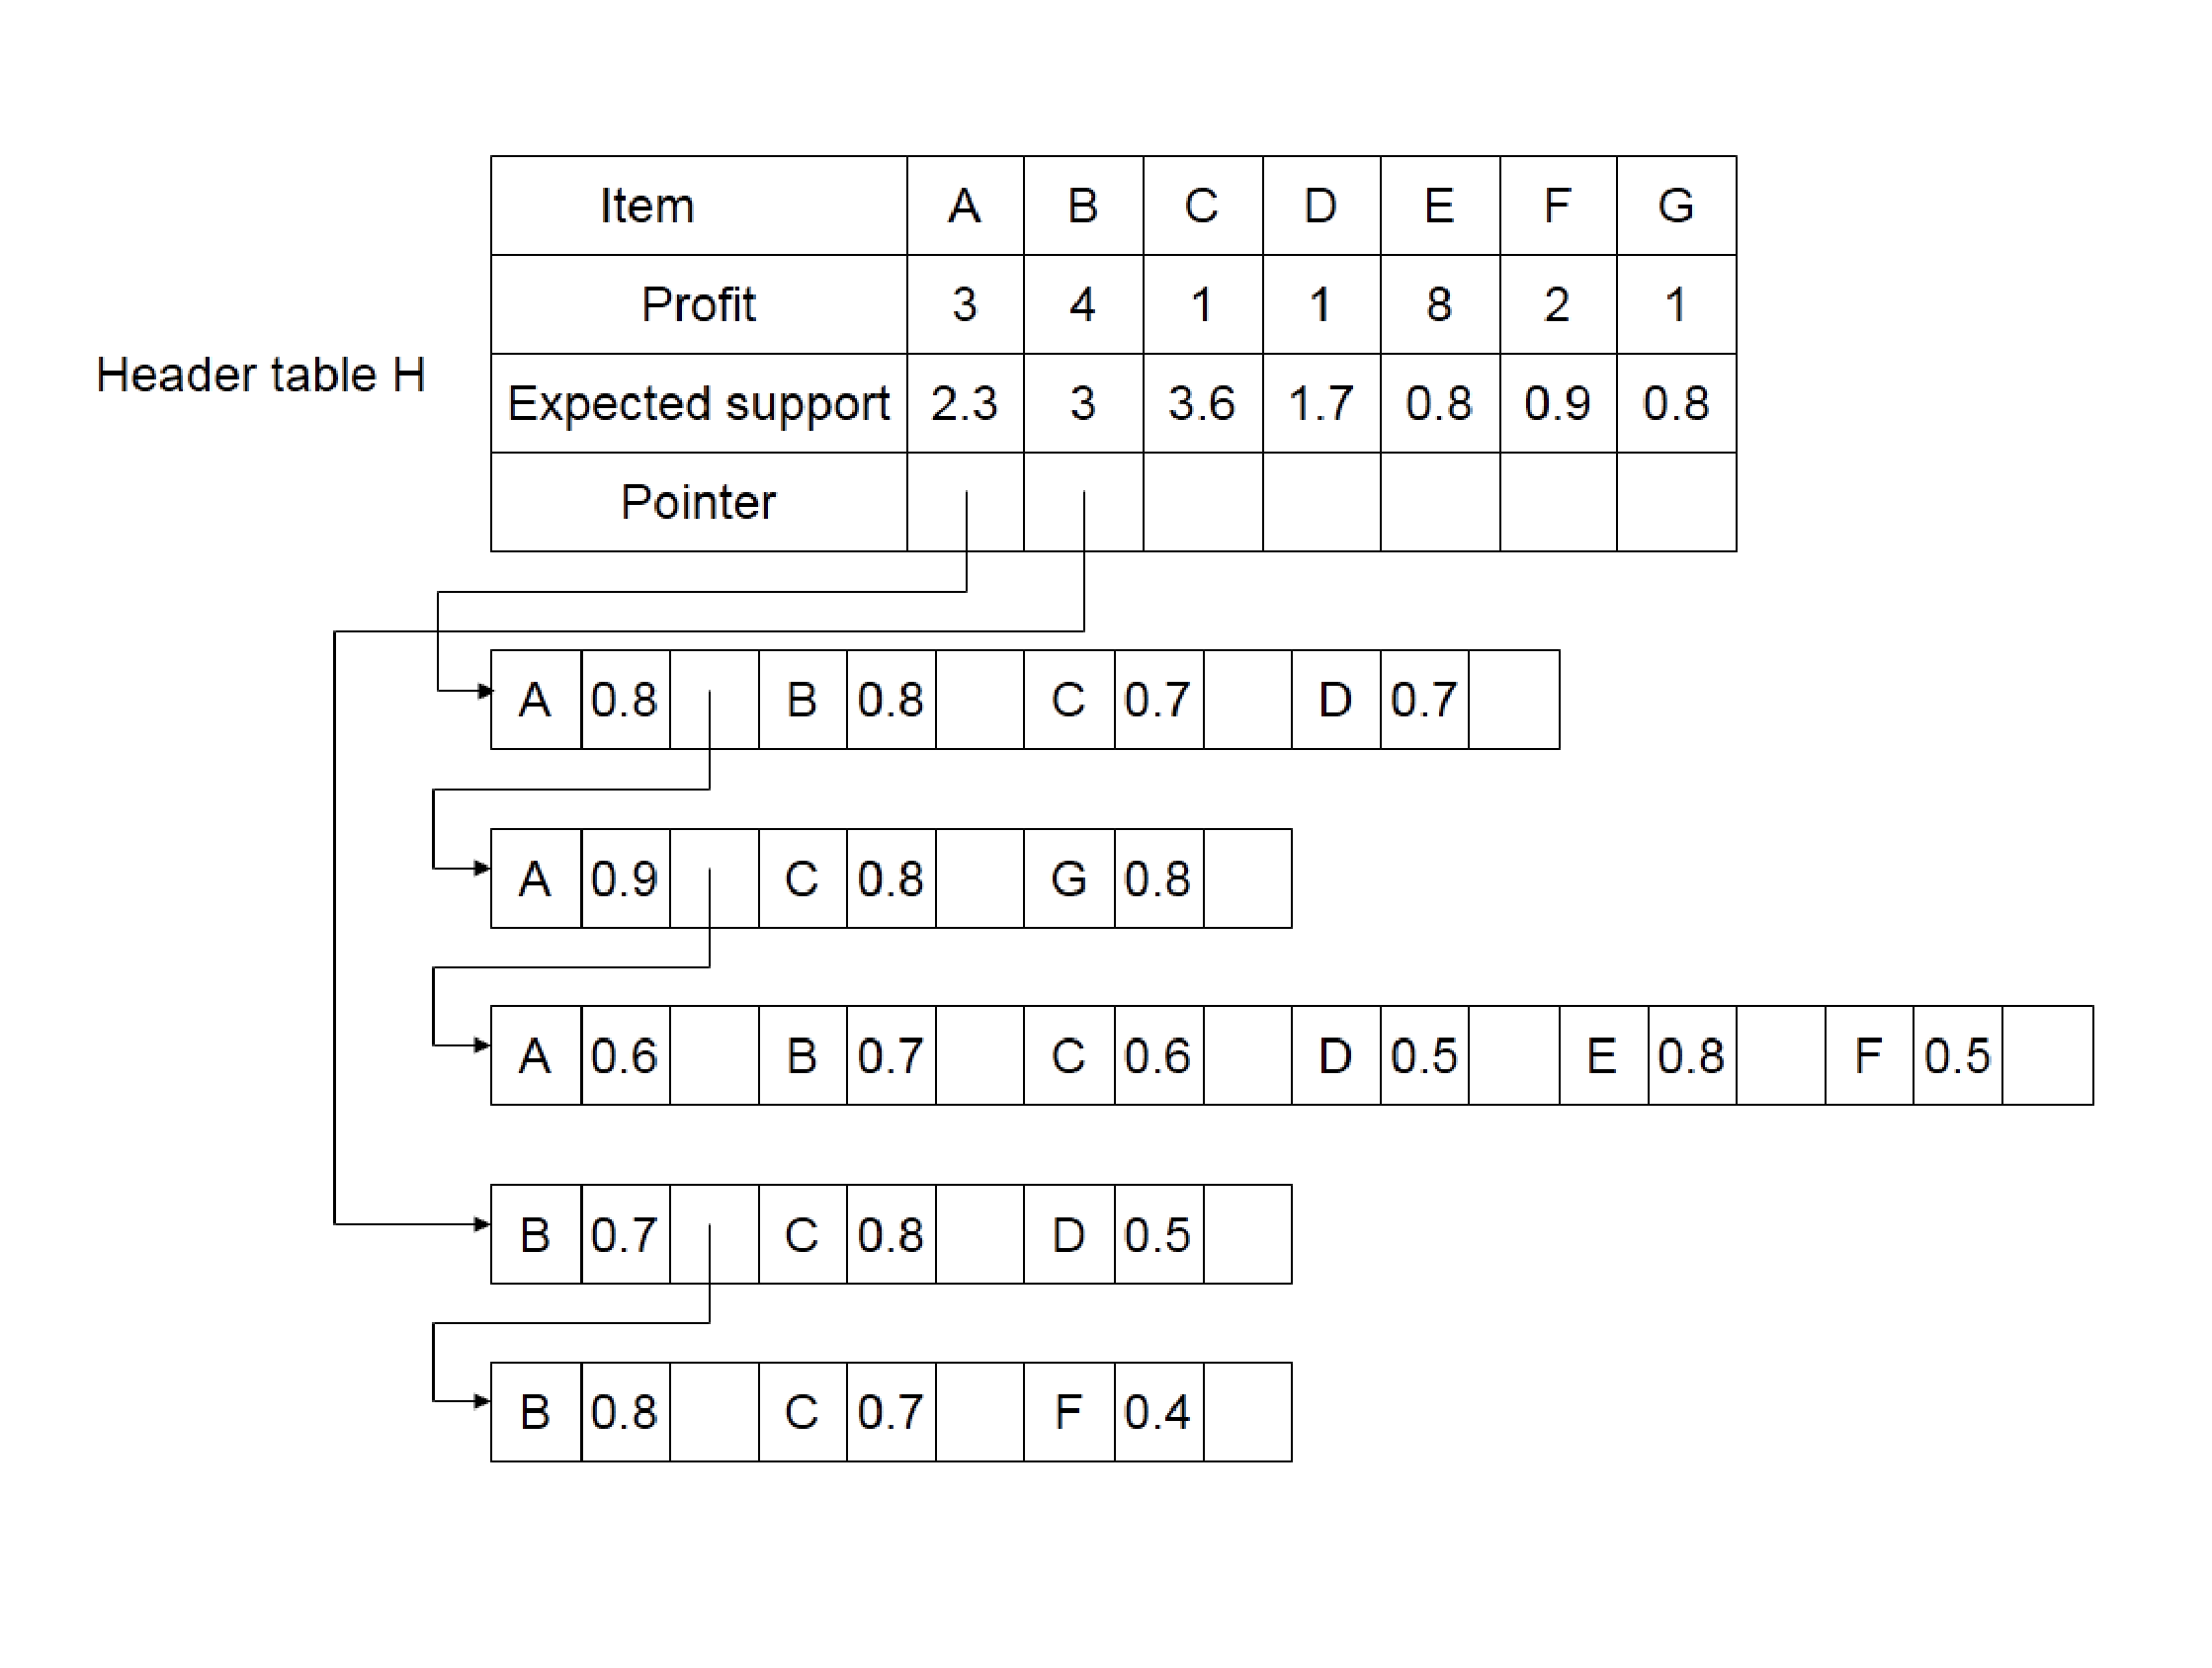
\includegraphics[width=0.99\textwidth]{1.eps}\\
  \caption{initial UUH-struct created from uncertain transaction database}
  \label{fig1}
\end{figure}

We can create a projection database through A-queue(which contains first, second and third transaction in Fig. \ref{fig2}. Then we can calculate profit and excepted support count of all 2-itemsets(such as $ {A, B} $, ${A, C}$) in projection database and create the header table $ H_{A} $(as shown in Fig. \ref{fig2}) and then link transactions to entries in header table $ H_{A} $. This structure can be traversed efficiently to find whether $ {A, B} $ is a high utility itemset.


\begin{figure}[htbp]
  \centering
  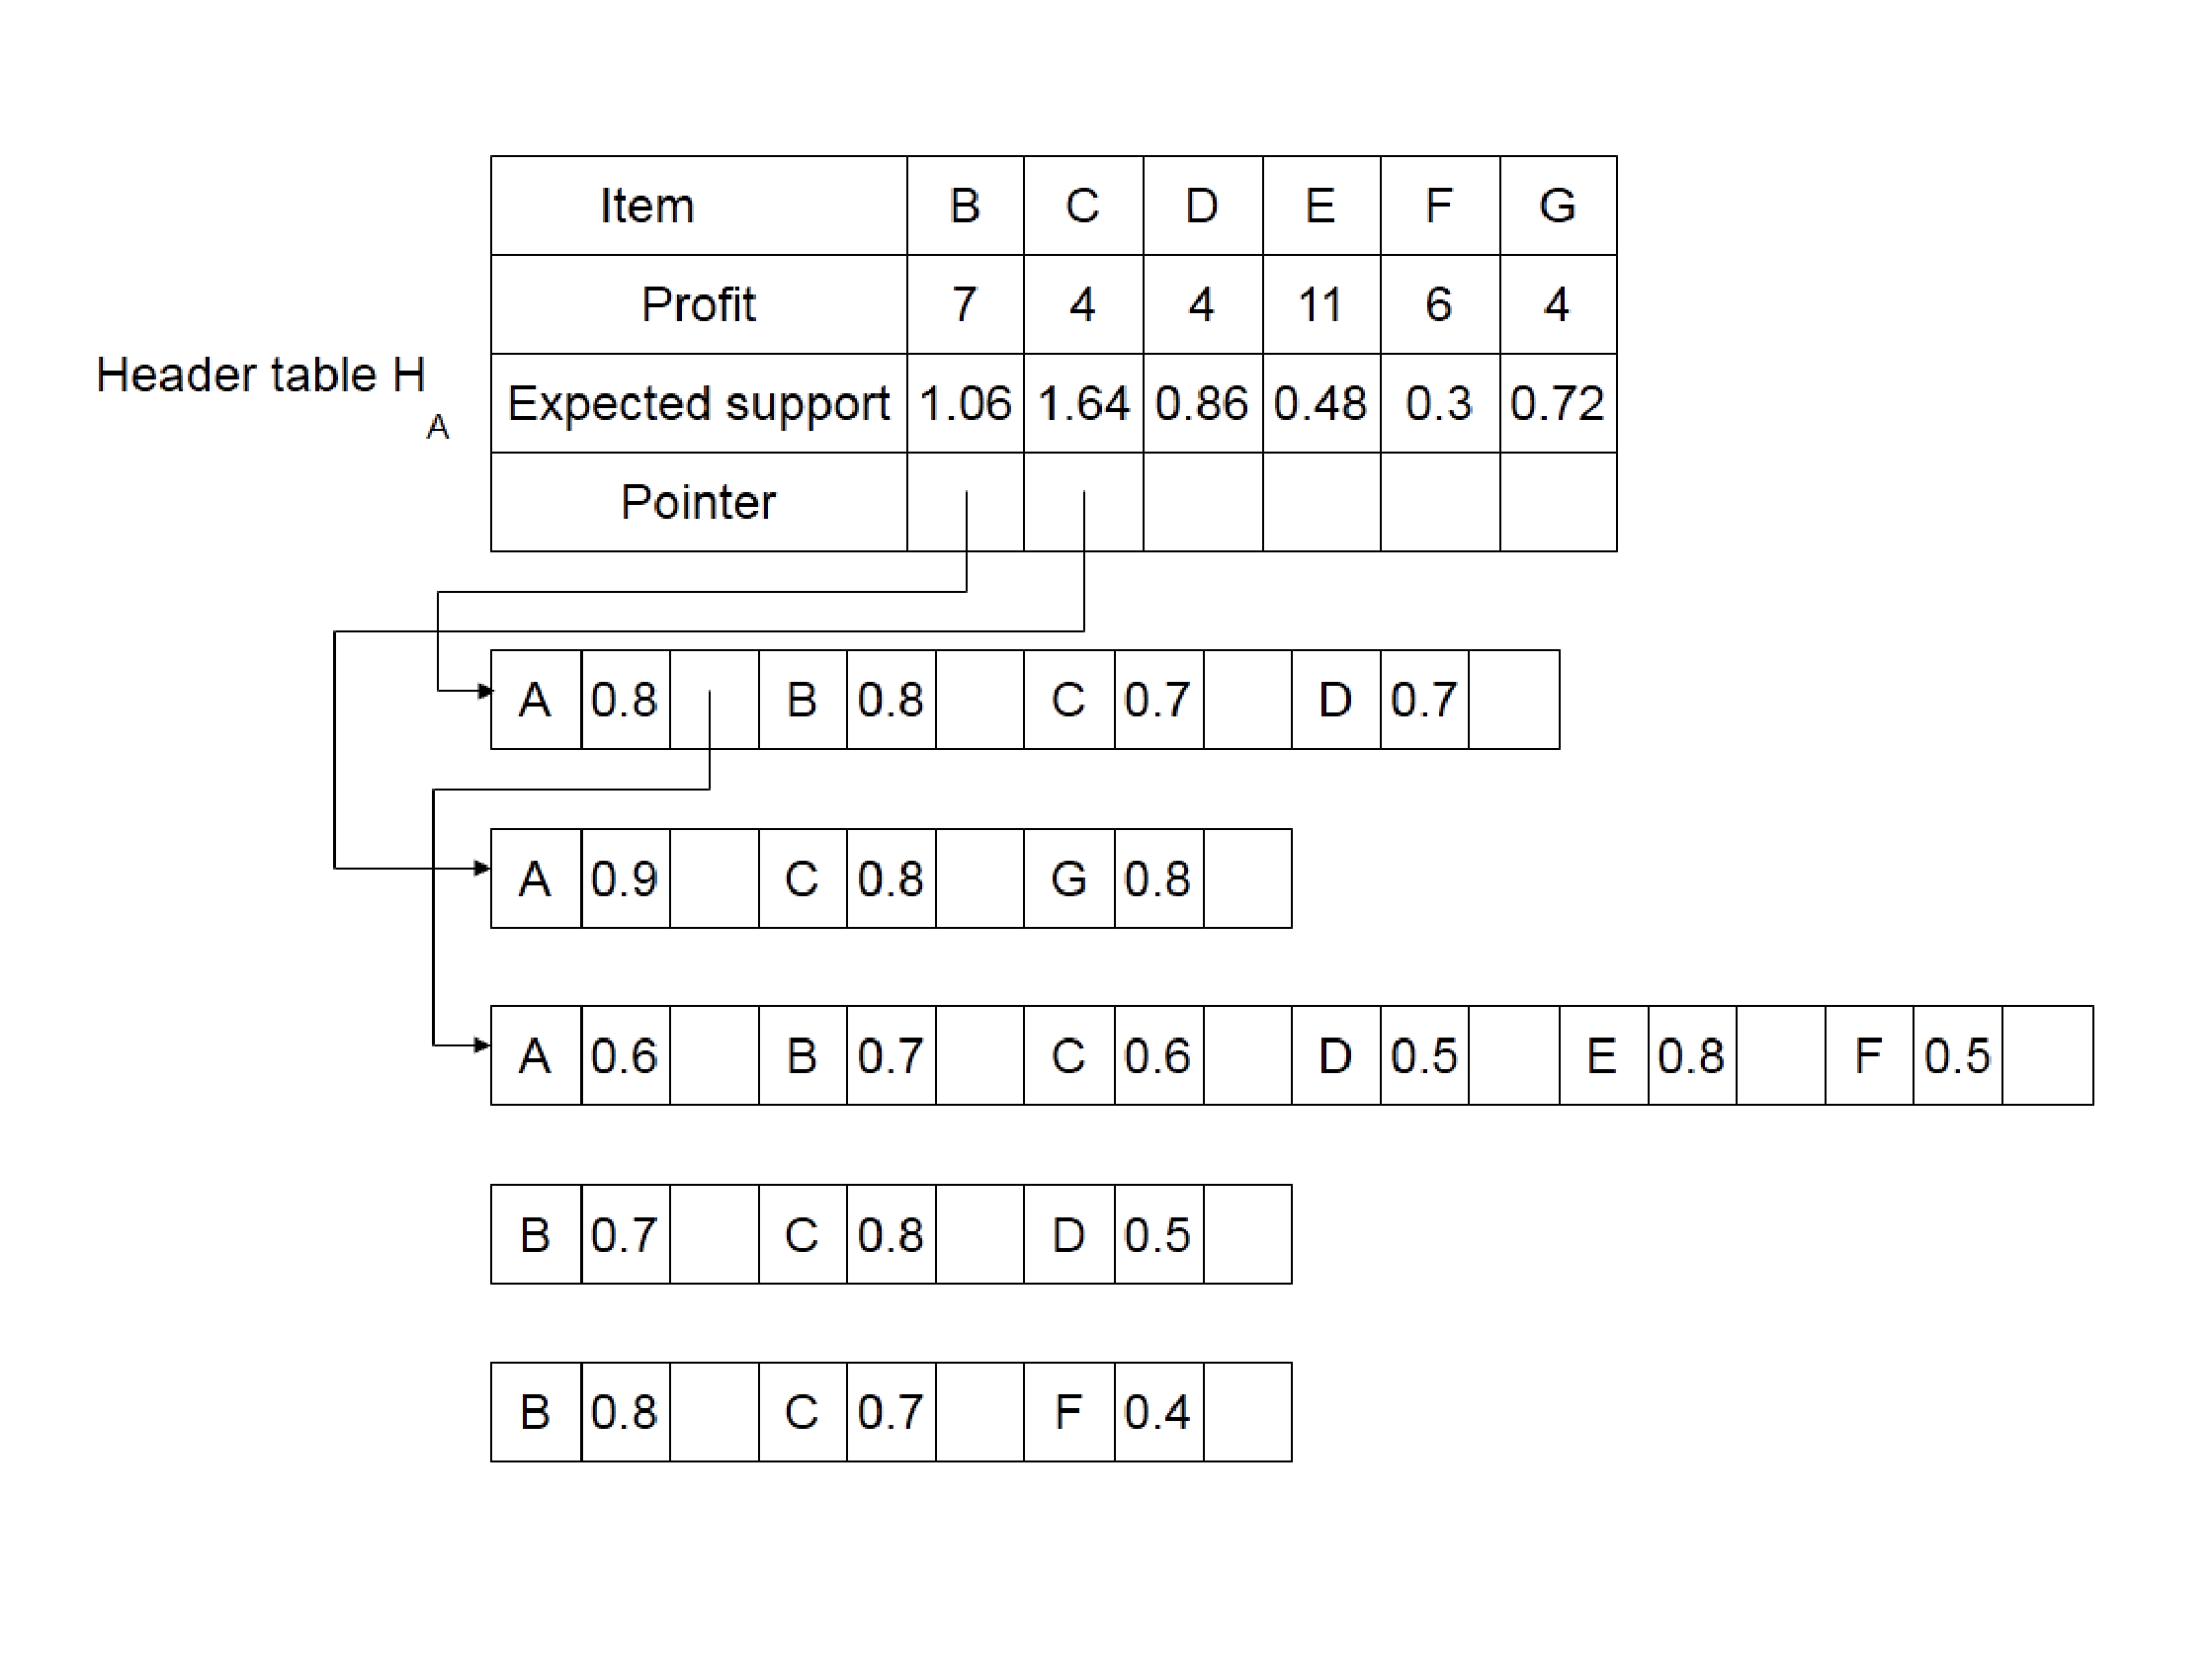
\includegraphics[width=0.99\textwidth]{2.eps}\\
  \caption{UUH-struct after creating header table $ H_{A} $}\label{fig2}
\vspace{-0.3cm}
\end{figure}

\begin{figure}[htbp]
  \centering
  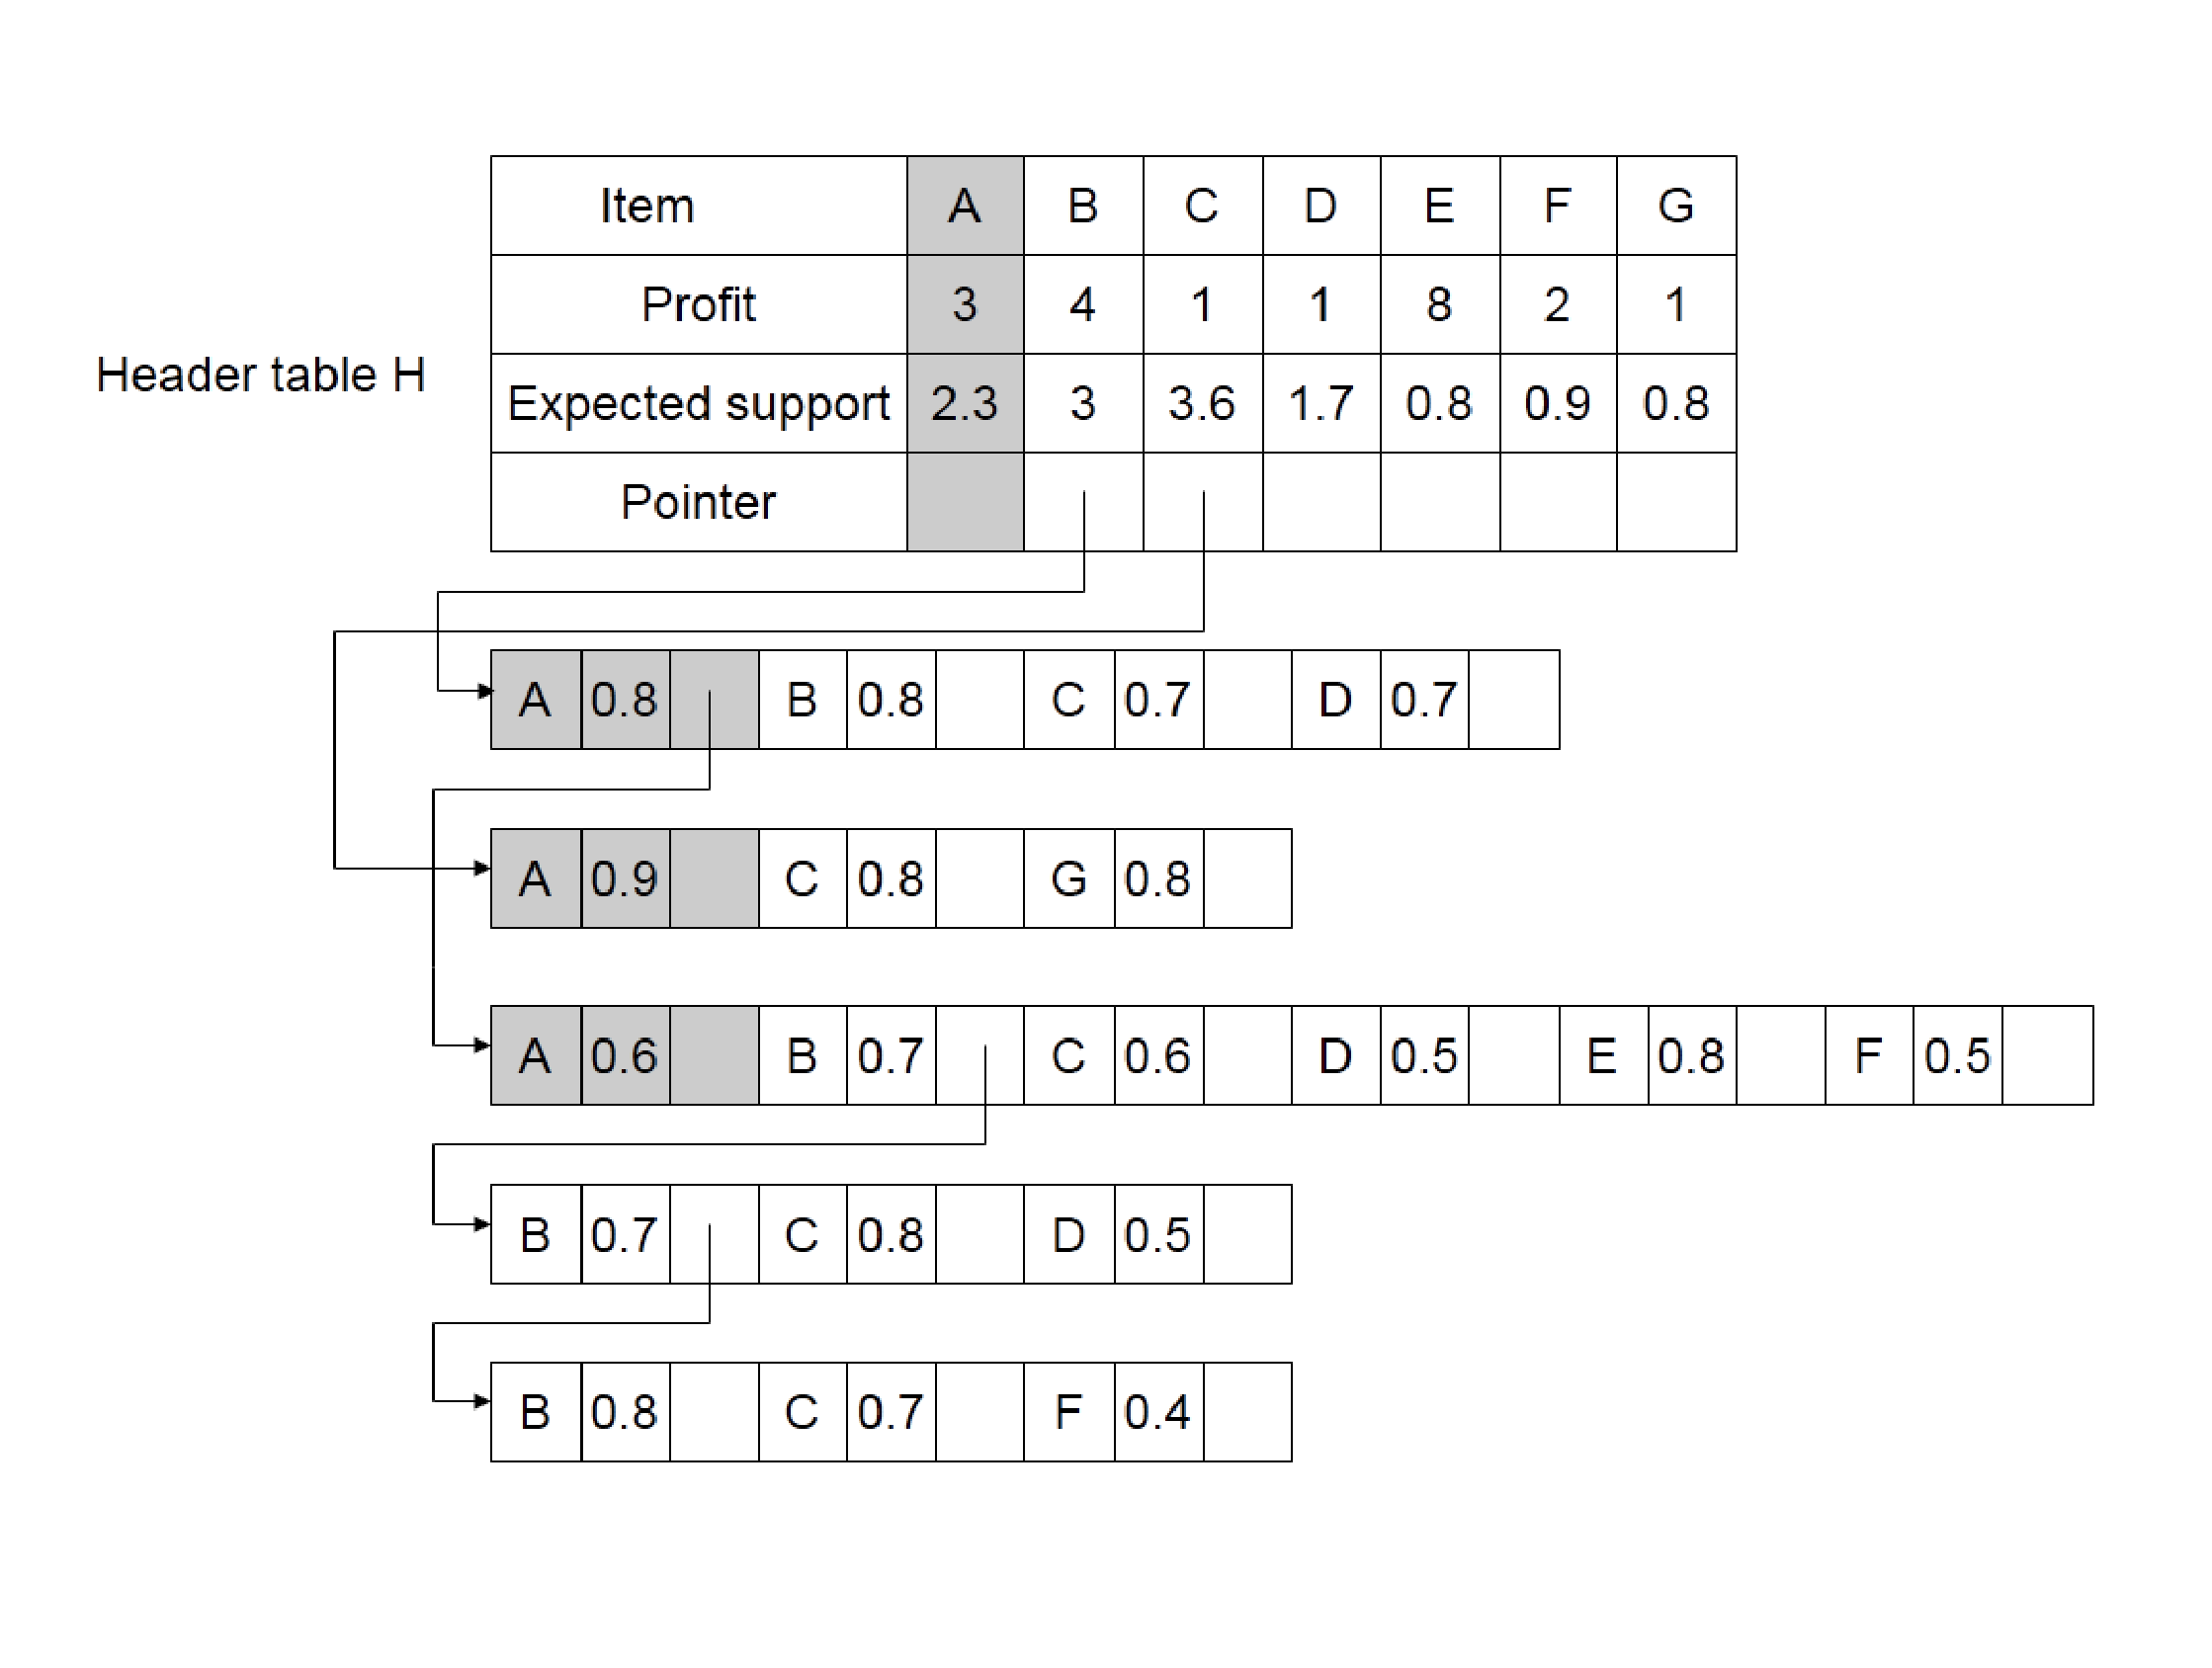
\includegraphics[width=0.99\textwidth]{3.eps}\\
  \caption{UUH-struct after removing item $ A $}\label{fig3}
\vspace{-0.3cm}
\end{figure}

Similarly, the process continues for the a-projected database and create header table $ H_{AB} $, $ H_{ABC} $...... to find high utility itemsets from all itemsets contaning $ A $. After high utility itemsets containing item $ A $ are found, the A-projected database, i.e., A-queue, is no longer needed for the remaining mining processes. So we delete item $ A $ from database and update the information in header table H(as shown in Fig. \ref{fig3}) to find high utility itemsets containing B.

We use UUH-mine framework to find all high utility itemsets from database through depth first search. However, this UUH-mine framework needs to traverse all $ 2^{m} $(m is the number of different items in database) itemsets to find the result, so we must optimize it.

\subsection{Algorithm optimization}

In this section, we will introduce the optimization scheme of UUH-mine framework.

\newtheorem{def10}[Rownumber]{Definition}
\begin{def10}
For the given uncertain transaction $ PT $, it's transaction maximum expected utility equals to the max expected utility of itemsets it contains, which is $ MU(PT)=max{U(I)|I\subseteq{PT}} $.
\label{def10}
\end{def10}

According to Definition \ref{def10}, we can add a new property to our example as shown in table \ref{utdeaamteu}.

\begin{table}[t]
\caption{Uncertain Database Adding Maximum Transaction Expected Utility}
\centering
{
\begin{tabular}{|c|c|c|}\hline
Index & Transaction content & Maximum transaction expected utility \\ \hline
1 & A(0.8), B(0.8), C(0.7), D(0.7) & 4.48 \\ \hline
2 & A(0.9), C(0.8), G(0.8) & 2.88 \\ \hline
3 & A(0.6), B(0.7), C(0.6), D(0.5), E(0.8), F(0.5) & 6.72 \\ \hline
4 & B(0.7), C(0.8), D(0.5) & 2.8 \\ \hline
5 & B(0.8), C(0.7), F(0.4) & 3.2 \\ \hline
\end{tabular}
}
\label{utdeaamteu}
\end{table}

The maximum expected utility of each transaction is calculated through it's content. For example, in table \ref{utdeaamteu}, the maximum expected utility of transaction 1 is 4.48, because the max expected utility of all 16 itemsets contained by transaction 1 is $ {A, B} $, which is 4.48.

In this example, the biggest transaction contains only 6 items, so we can calculate maximum expected utility of every transaction through exhaustive method. However, in practical problems, a transaction may contains many items,so the exhaustive method is not efficient. Here we will introduce a fast way:

Given a transaction PT which length(the number of items it contains) is $ L $, items in $ PT $ is $ i_{1}, i_{2}, ��, i_{L} $, probability of each item is $ p_{1}, p_{2}, ��, p_{L} $. We can give the sub problem $ S_{I,j} $($ i $ represent a itemset), which means the maximum expected utility in set which contains itemsets derived from itemset $ I $ and the last $ j $ items in $ PT $. Obviously we have $ EU(PT)=S_{\phi,L} $ and $ S_{I,0}=EU(I,PT) $ as well as recursive relation: $ S_{I,j}=max(S_{I\cup{i_{L-j+1}},j-1},S_{I, j-1}) $ (3.2). We can get $ EU(PT) $ from that recursive relation, but it still need to consider all $ 2^{L} $ itemsets. So we can use this theorem to optimize it:

\newcounter{Theoremnumber}

\newtheorem{the1}[Theoremnumber]{Theorem}
\begin{the1}
If there exist itemset $ I_{1} $ and $ I_{2}=I_{1}\cup{i_{j}} $ ($ I_{2} $ represents a superitemset which has one more item than $ I_{1} $), and meet $ EU(I_{1},PT)\>EU(I_{2},PT) $, then expected utilities of $ I_{2} $ and all superitemsets of $ I_{2} $ cannot be the maximum expected utility of $ PT $.
\label{the1}
\end{the1}

\newcounter{Rationalenumber}

\newtheorem{ra1}[Rationalenumber]{Rationale}
\begin{ra1}
The expected utility of $ I_{2} $ obviously cannot be the maximum expected utility of $ PT $, so we will prove that is also true for $ I_{2} $'s superitemsets $ I_{3}=I_{2}\cup{I^{'}} $. For one of $ I_{2} $'s superitemset , we can construct a new itemset $ I_{4}=I_{1}\cup{I^{'}} $, then we have

{\setlength\arraycolsep{1pt}
\small
\begin{eqnarray}
\label{eq:egSPr}
\ & EU(I_{3},PT) & = U(I_{3})\times{Pr(I_{3},PT)}
\nonumber \\
&&{} =(U(I_{2})+U(I^{'}))\times{Pr(I_{2},PT)}\times{Pr(I^{'},PT)}
\nonumber \\
&&{} =(EU(I_{2},PT)+U(I^{'})\times{Pr(I_{2},PT)})\times{Pr(I^{'},PT)}
\end{eqnarray}}

{\setlength\arraycolsep{1pt}
\small
\begin{eqnarray}
\label{eq:egSPr}
\ & EU(I_{4},PT) & =U(I_{4})\times{Pr(I_{4},PT)}
\nonumber \\
&&{} =(U(I_{1})+U(I^{'}))\times{Pr(I_{1},PT)}\times{Pr(I^{'},PT)}
\nonumber \\
&&{} =(EU(I_{1},PT)+U(I^{'})\times{Pr(I_{1},PT)})\times{Pr(I^{'},PT)}
\end{eqnarray}}

because $ EU(I_{1},PT)>EU(I_{2},PT) $ and $ Pr(I_{1},PT)\ge{Pr(I_{2},PT)} $, so $ EU(I_{3},PT)<EU(I_{4},PT) $, so the expected utility of $ I_{3} $ cannot be the maximum expected utility of $ PT $.


\label{ra1}
\end{ra1}

We can use Theorem. 1 to  optimize Eq. \ref{eq1}:

\begin{equation}
\label{eq1}
\small{
S_{i,j}=\begin{cases}
max\{S_{I\cup{\{i_{L-j+1}\},j-1}},S_{I,j-1}\} & (EU(I,PT)<EU(I\cup{\{i_{L-j+1}\},PT})) \\
S_{I,j-1} & (EU(I,PT)\ge{EU(I\cup{\{i_{L-j+1}\},PT}))}
\end{cases}
}
\end{equation}

Using Eq. \ref{eq1} can greatly speed up the calculation of transaction maximum expected utility.

\newtheorem{def11}[Rownumber]{Definition}
\begin{def11}
For itemset $ I $ and uncertain transaction database $ UD $, the transaction maximum expected utility of itemset $ I $ is $ MU(I)\sum\limits_{I\subseteq{PT\land{PT\in{UD}}}}MU(PT) $. Which means the sum of transaction maximum expected utility of transactions containing itemset $ I $.
\label{def11}
\end{def11}

\newcounter{Lemmanumber}

We can derive Lemma \ref{lem1} through definitions above:

\newtheorem{lem1}[Lemmanumber]{Lemma}
\begin{lem1}
The transaction maximum expected utilities of $ I $'s superitemsets are not more than $ I $'s. For $ I\subseteq{I^{'}} $, there always have $ MU(I)\le{MU(I^{'})} $.
\label{lem1}
\end{lem1}

According to Chernoff bound\cite{bib2}, random variables $ X_{1}, X_{2}, ��, X_{n} $ are results of n times independent Poisson experiments($ X_{j} $ can only be $ 0 $ or $ 1 $). Given $ X=\sum_{j=1}^{n}{X_{j}} $ and$ \mu=E[X] $, for any positive read number $ \delta $, there exists the following inequality:

\vspace{-0.2cm}
\begin{equation}
\label{eq2}
\small{
Pr(X\le{(1+\delta)\mu})<\{\frac{\mathrm{e}^{\delta}}{(1+\delta)^{1+\delta}}\}^{\mu}  (\delta>0)
}
\end{equation}

In the problem of mining probabilistic high utility itemsets, for one itemset $ I $, it's appear in one uncertain transaction $ PT $ can be seen as a independent Possion experiment, and the real support of $ I $, I.e. the $ sup(I) $ is the sum of many Possion experiments, so the expect of that variable is the expected support count of $ I $. So the utility probability of $ I $ we need to calculate is:

\begin{equation}
\label{eq3}
\small{
Pr(sup(I)\times{U(I)}\ge{minutil})=Pr(sup(I)\ge{\frac{minutil}{U(I)}})
}
\end{equation}

Combine Eq. \ref{eq2} and Eq. \ref{eq3}, when $ esupp(I)<\frac{minutil}{U(I)} $, we can let $ (1+\delta)esup(I)=\frac{minutil}{}U(I) $,  so we can get $ \delta=\frac{minutil}{U(I)esup(I)}-1=\frac{minutil}{EU(I)}-1 $. Feed it into Eq. \ref{eq2} can get:

\begin{equation}
\label{eq4}
\small{
Pr(up(I)\ge{minutil})<(\frac{\mathrm{e}^{\delta}}{(1+\delta)^{1+\delta}})^{esup(I)}
}
\end{equation}

while $ \delta=\frac{minutil}{EU(I)}-1 $.The right side of inequality \ref{eq4} is a decreasing function of $ \delta $, so when $ \delta $ decreases, the original inequality still holds. Hence we can get the following Lemma:

\newtheorem{lem2}[Lemmanumber]{Lemma}
\begin{lem2}
For itemset $ I $, given uncertain transaction database $ UD $, utility threshold $ minutil $ and probabilistic utility threshold put, if $ MU(I)<minutil $ and $ (\frac{\mathrm{e}^{\delta}}{(1+\delta)^{1+\delta}})^{esup(I)}\le{put} $ (where $ \delta=\frac{minutil}{MU(I)}-1 $), then itemset $ I $ and all of it's superitemsets cannot be utility itemsets.
\label{lem2}
\end{lem2}

\vspace{-1cm}
\begin{figure}[t]
  \centering
  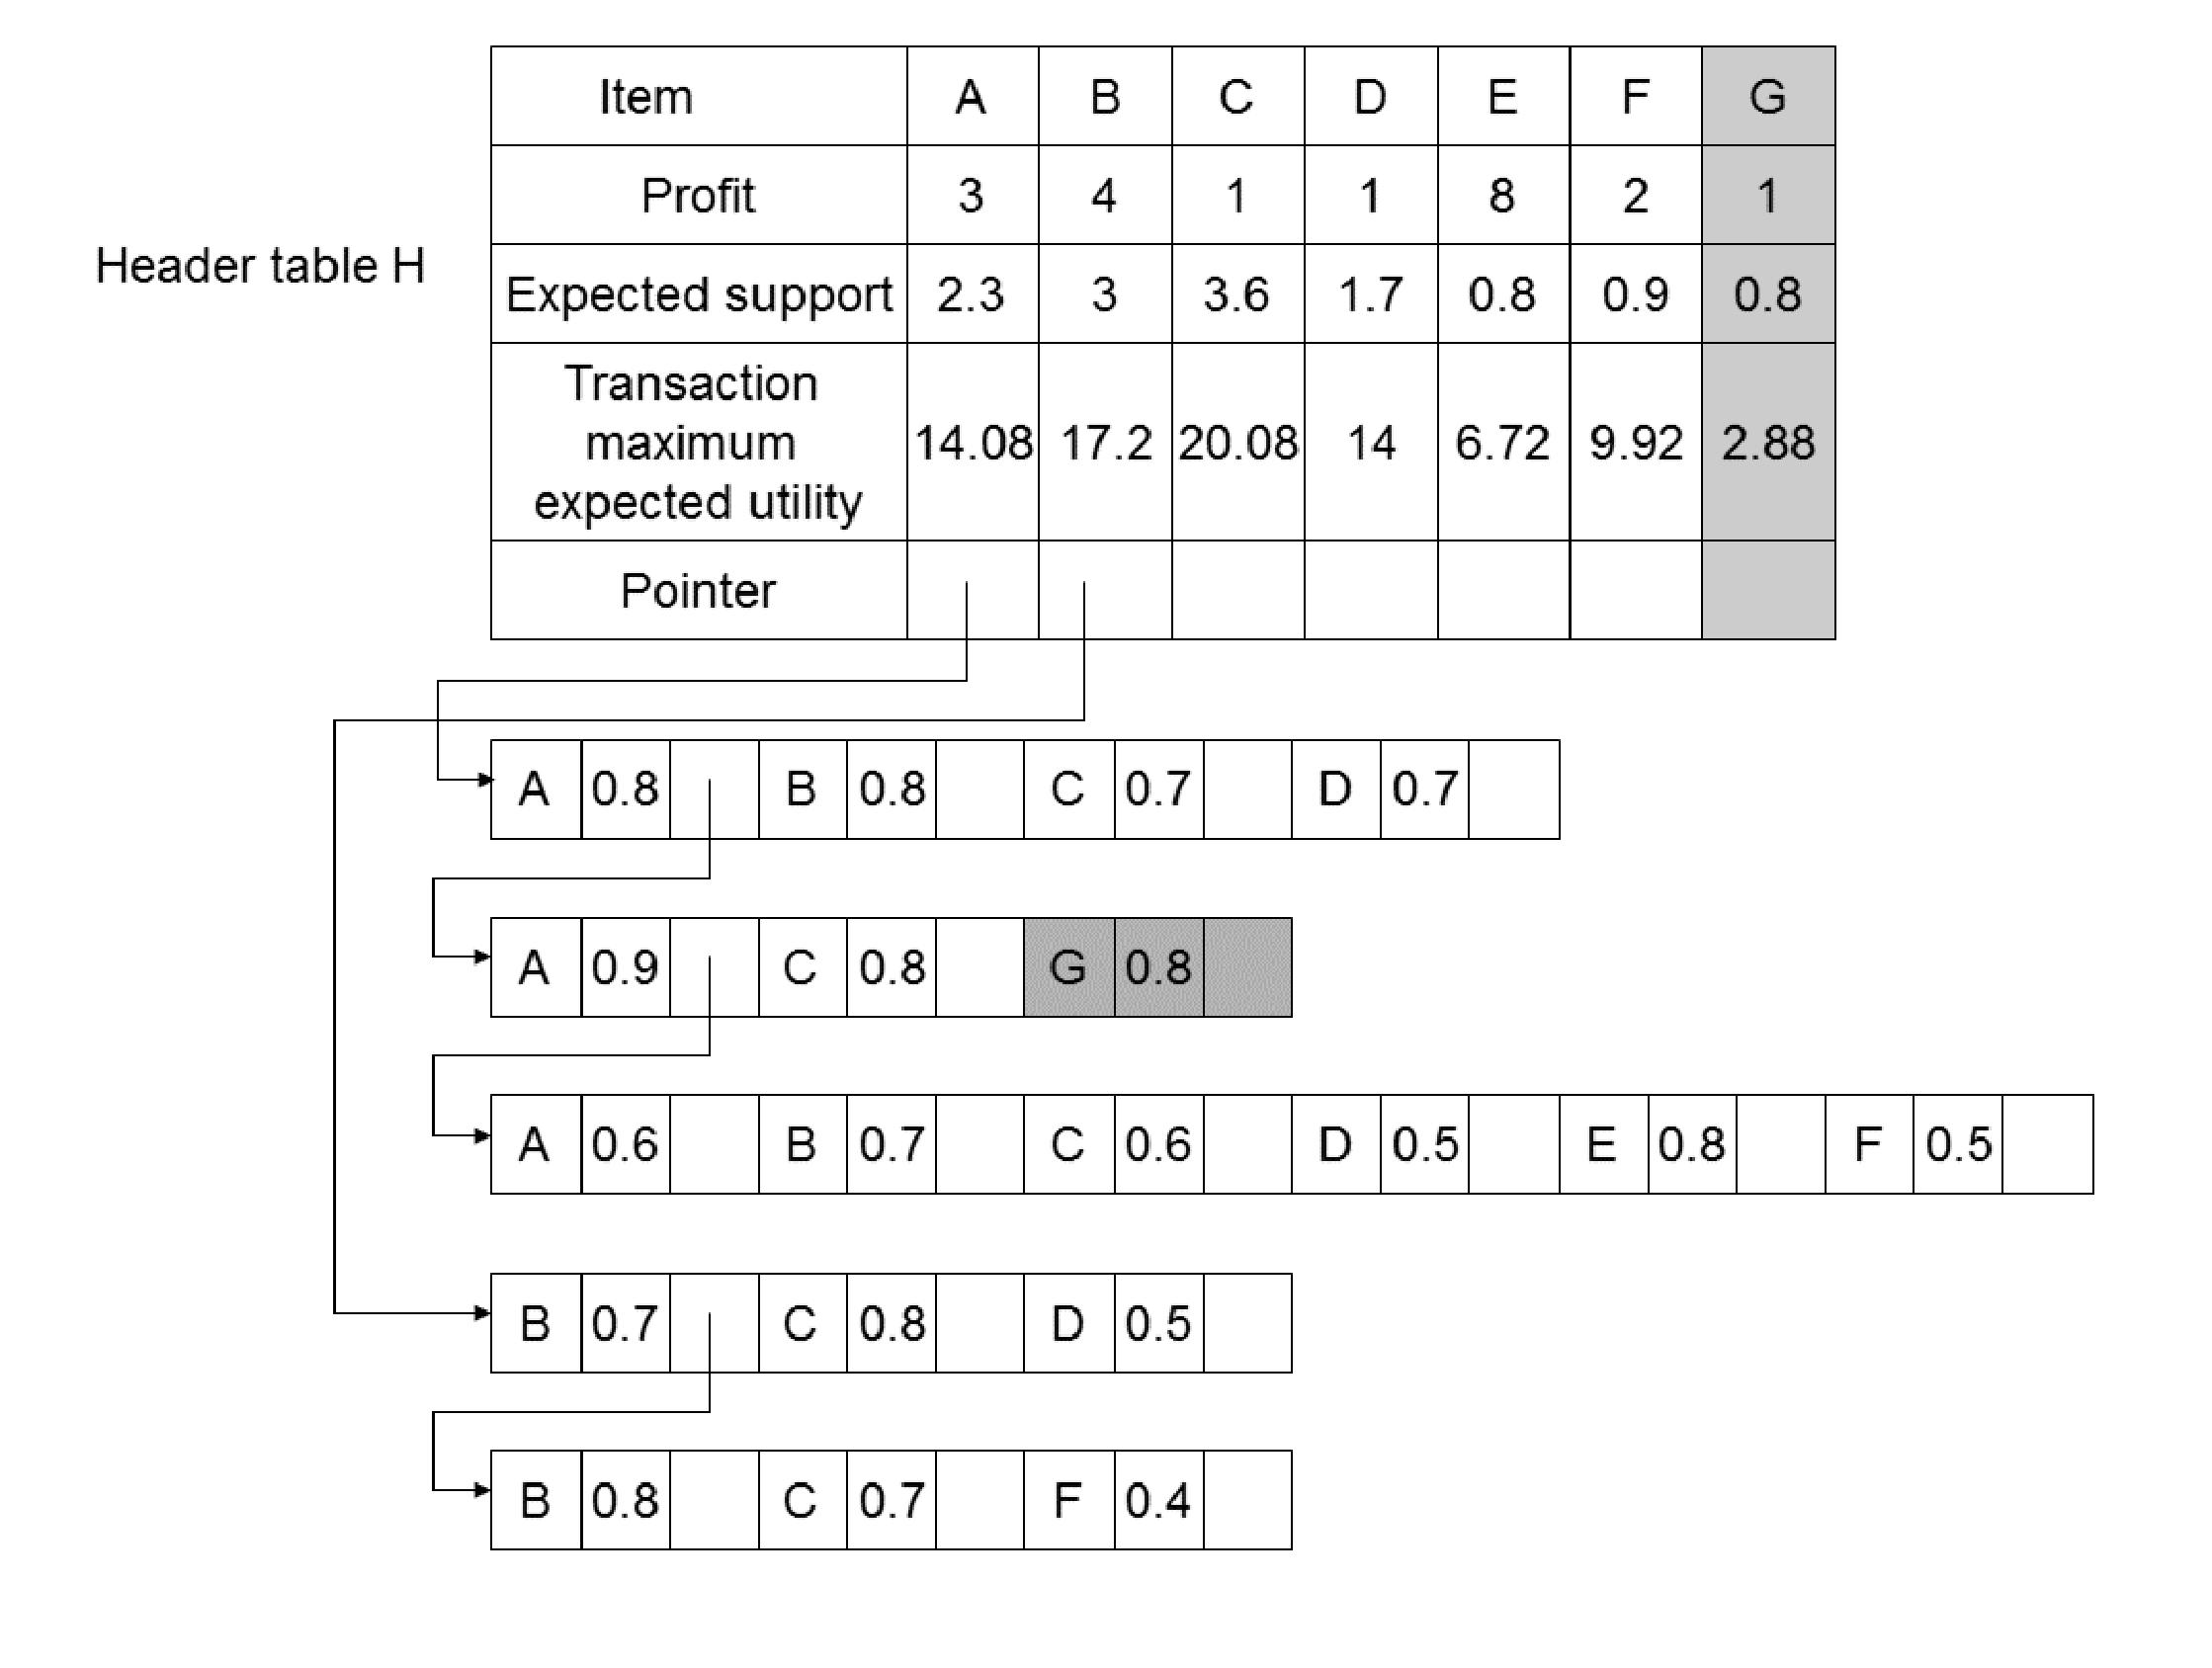
\includegraphics[width=0.99\textwidth]{4.eps}\\
  \caption{initial UUH-min data structure after optimization}\label{fig4}
  \vspace{-0.3cm}
\end{figure}

Lemma \ref{lem2} is the key point to solve the``uncertain database utility itemset minin'' problem, it can greatly reduce the search space so that the algorithm can be efficient. We can use it to optimize the UUH-mine framework mentioned in last section, as shown in Fig. \ref{fig4}. Because the transaction maximum expected utility of itemset $ {G} $ is 2.88, cannot pass the check in Lemma \ref{lem2}, so $ {G} $ and all of it's superitemsets cannot be utility superitemsets and we don't need to check them.

Of course, we can use the same method to optimize the other header tables generated by projection databases(such as $ H_{A}, H_{AB} $, etc).

\subsection{UUIM algorithm}

In this section, we will introduce UUIM(Uncertain Utility Itemsets Mining) algorithm in detail. First, we will give the overall outline of this algorithm, which divides the mining process into two phases and briefly describe them. Then we will explain that two phases in detail.

\begin{algorithm}[htbp]
  \small{
  \caption{\small{UUIM Algorithm}}
  \label{alg:uuim}
  \KwIn{uncertain transaction database $ UD $, utility threshold $ minutil $, probabilistic utility threshold $ put $}
  \KwOut{set of utility itemset $ UIS $}
  UIS��\;
  \emph{H��InitializeHeader(UD, minutil, put)}\;
    \emph{Recursion(H, UD, minutil, put, UIS)}\;
  return UIS}
\end{algorithm}

Algorithm 1(UUIM) is the algorithm framework of mining utility itemsets. This algorithm is purposed to mine all utility itemsets $ UIS $ from the given uncertain transaction database UD through the given utility threshold minutil and probabilistic utility threshold put. Line 1 is used to initialize the result set $ UIS $; line 2 creates the initial header table H of the UUH-mine framework through function InitializeHeader; line 3 use the key function Recursion search each items in depth first way; the last line return the calculation results which are all utility itemsets. According to this we can know that the main part of this algorithm consists of two parts, one for creating header table which is explained above in detail; the other is the recursive function Recursion which is used to traverse all probabilistic utility itemsets.

Next, we will introduce how the key function  Recursion works. In algorithm 2(Recursion), line 1 traverses each itemset in header table; line 2 and 3 check whether the new itemset   is utility itemset, if true it will be added to result; line 4 checks whether that new itemset can pass the Eq. (3.6), if passed a header table will be created in line 5 and traversed in line 6.

\begin{algorithm}[htbp]
  \small{
  \caption{\small{Recursion Algorithm}}
  \label{alg:recursion}
  \KwIn{header table $ H_{I} $, uncertain transaction database $ UD $, utility threshold $ minutil $, probabilistic utility threshold $ put $, current set of utility itemset $ UIS $}
  \KwOut{updated set of utility itemset $ UIS $}
  \For{each $ i $ in $ H_{I} $ do}{
  \If{$ I\cup{i} $ is utility itemset do}{
    $ UIS=UIS\cup{I\cup{i}} $
  }
  \If{ChernoffCheck($  $) = true do}{
    \emph{create new header table $ H_{I\cup{i}} $}\;
    \emph{Recursion($ H, UD, minutil, put, UIS $)}\;
  }
  }
  End;}
\end{algorithm}



In summary, this section explains the probabilistic utility itemset mining algorithm, UUIM. First we introduce a new data structure UUH-struct, which lay the foundation of the algorithm's efficiency; then we describe several algorithm optimization methods such as global bound and local pruning in order to speed up the algorithm.

\section{Experimental evaluation}

Experiments are performed to test the effectiveness of our UUIM algorithm in obtaining the high utility transactions. First we will introduce the software platform, hardware platform, datasets, variable setting rules and the experiment; then the effectiveness of UUIM will be considered through it's running time, especially with Chernoff pruning strategy; next the memory cost of UUIM will be compared and finally, we will conclusion this section.

\subsection{Introduction to experiment platform}


All experiments were performed on a Intel(R) Core(TM) i5 M450 2.40GHz PC machine with 4GB main memory, running Microsoft Windows 8.1. UUIM was implemented by us using C++ in Visual Studio 2012.

In order to ensure the fairness of experiment, according to the experimental evaluation method of probabilistic database research field in previous, we will assign probability to transactions in real certain transaction database to get an uncertain transaction database. The way we used for assigning is assign a probability value to one transaction, the value obey the normal distribution given expected and variance. We use the classical transaction database Mushroom which comes from Audobon Society Field Guide and contains 8124 transactions and 120 different items.

Given experiment platform, we will further explain the evaluation scheme. The evaluation scheme consists of two parts, the algorithm efficiency evaluation and the memory cost evaluation. During the evaluation progress, we mainly compare the efficiency of UUIM algorithm and UUIM-NoCh algorithm. The UUIM-NoCh algorithm didn't use the Chernoff pruning strategy. According this comparison we can verify the validity of that strategy.

Besides, the main variables used in UUIM are utility threshold minutil and probabilistic utility threshold put, so the following two experiments will show the influence of these two variables to UUIM algorithm and Chernoff bound pruning strategy. The following are the experiment results.


\subsection{Algorithm efficiency evaluation}

Based on the experiment scheme in last section, this section mainly evaluate the  algorithm efficiency. We will evaluate from three angles: change of utility threshold, change of probabilistic utility threshold and whether use Chernoff bound pruning strategy. In order to hold the principle of single variable, the default parameter setting is: default utility threshold minutil = 10000, default probabilistic utility threshold put = 0.6. When one of them is changing, the other keep the default value. Moreover, the range of the utility threshold minutil is 5000 to 15000 while the range of the probabilistic utility threshold put is 0.5 to 0.9. According these big ranges, we can clearly see the characteristics of UUIM algorithm and UUIM-NoCh algorithm thus the presented experiment results can be more objective.

Fig. \ref{fig5} shows the comparison of UUIM algorithm and UUIM-NoCh algorithm in different utility threshold. Clearly, in the same parameter setting the efficiency of UUIM algorithm is about two times more than the efficiency of UUIM-NoCh algorithm. And the difference becomes lager as the utility threshold goes lower. This shows that the Chernoff bound pruning strategy can efficiently reduce the search space, greatly decrease the number of itemsets need to be calculated, thus greatly increase the algorithm efficiency.

\begin{figure*}[htbp]
  \centering
  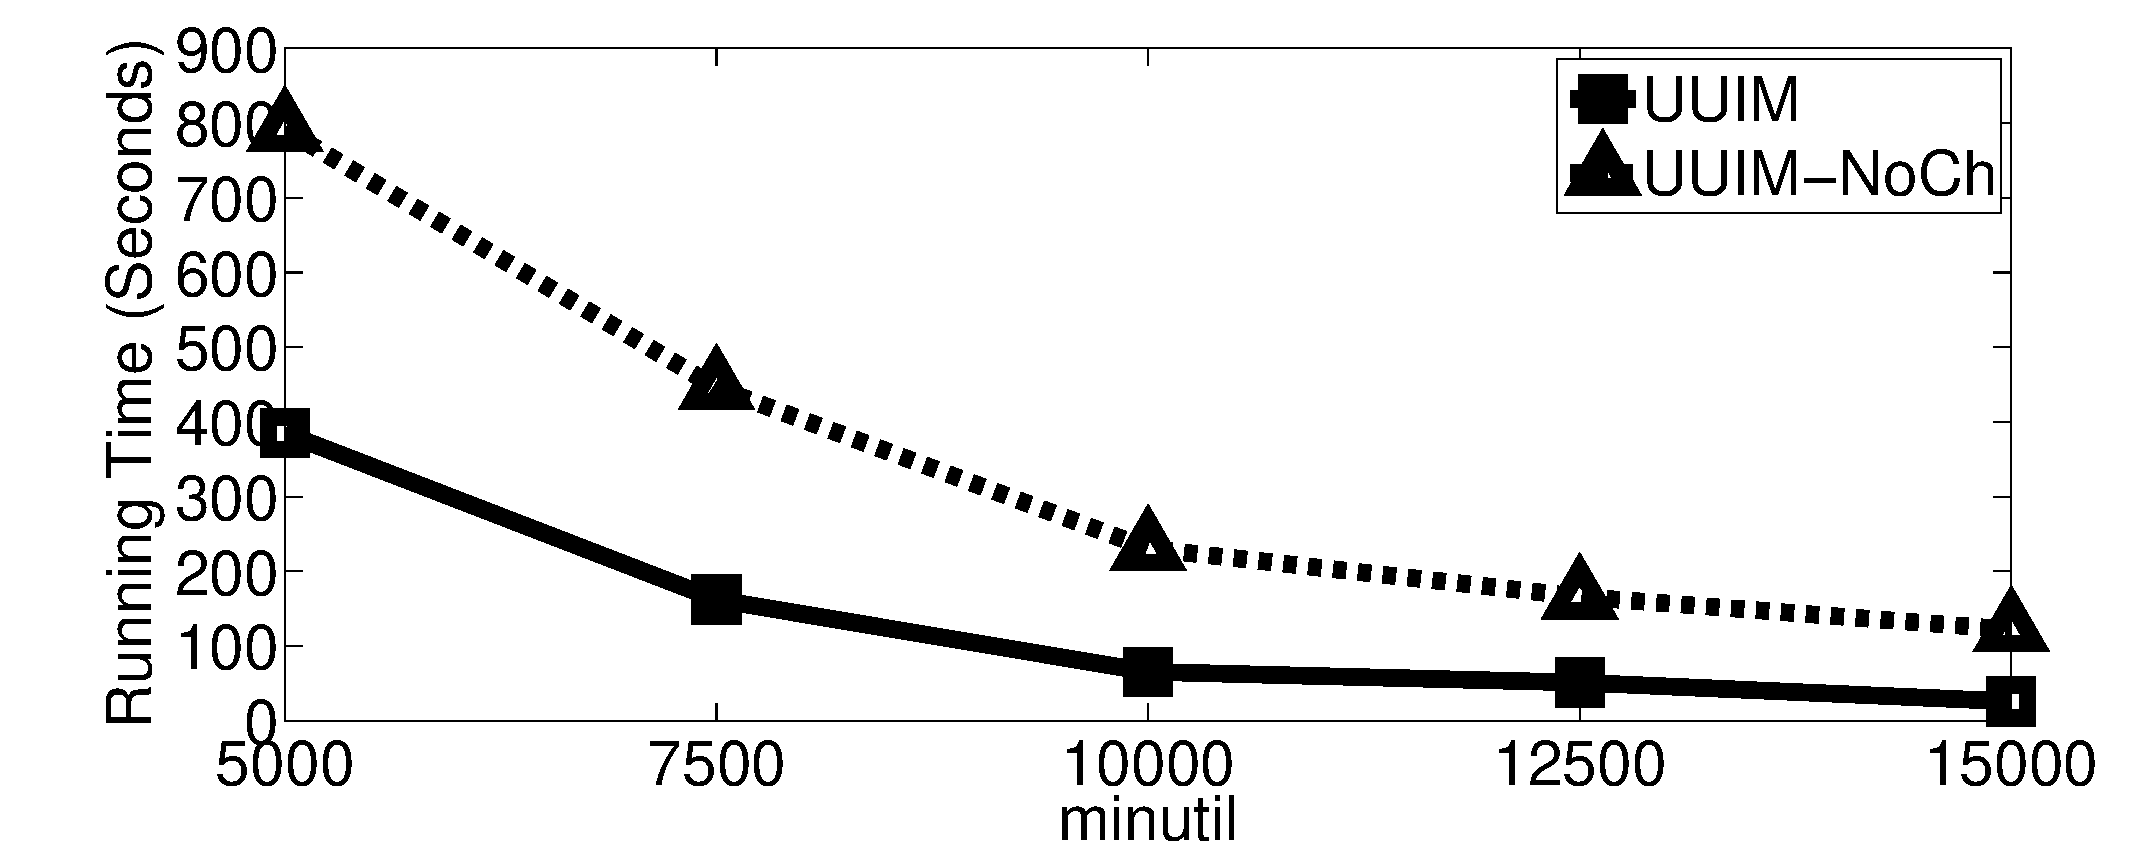
\includegraphics[width=0.99\textwidth]{5.eps}\\
  \caption{Running Time vs. Minimum Utility Threshold}\label{fig5}
  \vspace{-0.3cm}
\end{figure*}

Then we test the influence of the change of probabilistic utility threshold to UUIM algorithm and UUIM-NoCh algorithm. Fig. \ref{fig6} shows that while the probabilistic utility goes higher, the running time of UUIM-NoCh left largely unchanged, but the running time of UUIM algorithm is decreasing. Thus shows that while the probabilistic utility threshold gets higher, the effect of Chernoff bound pruning strategy will be better, but it does not influence UUIM-NoCh algorithm.

\begin{figure}[htbp]
  \centering
  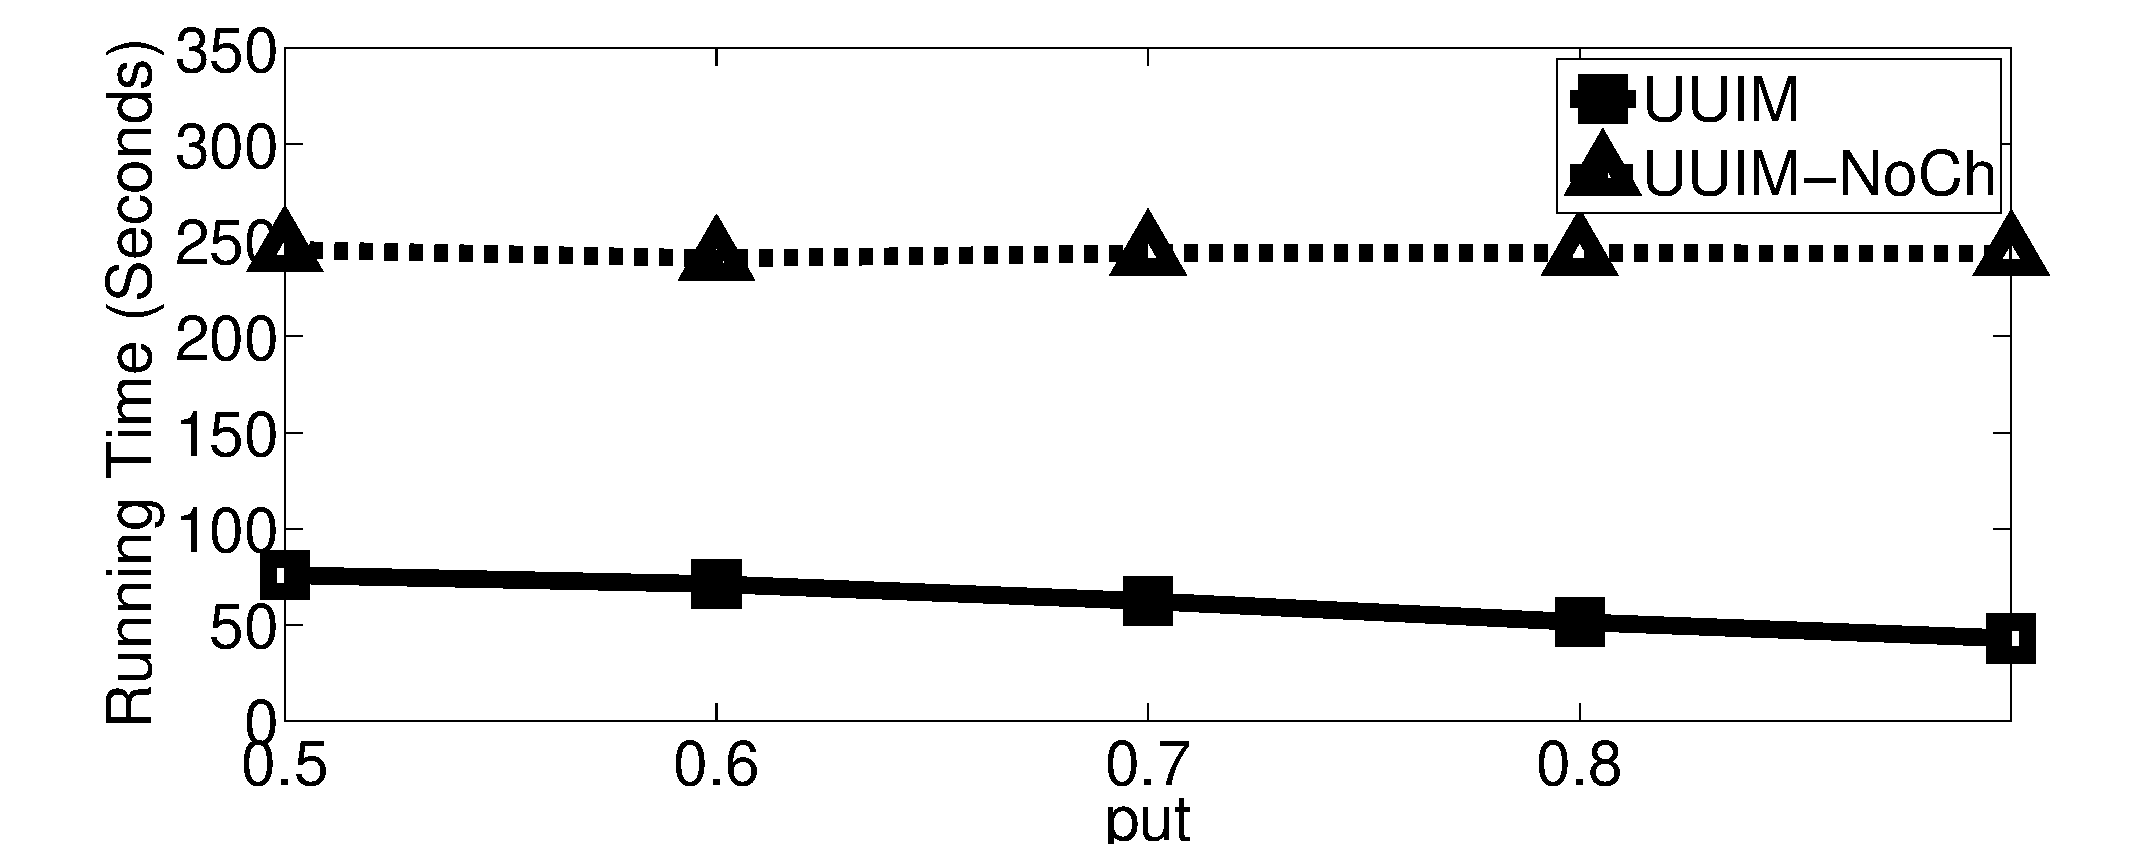
\includegraphics[width=0.99\textwidth]{6.eps}\\
  \caption{Running Time vs. Probabilistic Uility Threshold}\label{fig6}
  \vspace{-0.3cm}
\end{figure}

\subsection{Memory cost evaluation}

Based on the experiment scheme, this section mainly evaluate the memory cost of the algorithm. During this process, we will mainly compare the peak memory cost. As mentioned in section 3, UUH-struct in UUIM algorithm need many header tables to store the transaction maximum utility of each itemset in order to use the pruning strategy. So we will focus on whether we can control the increase extant of memory cost.

Similar to last experiment, the default utility threshold is minutil=10000 and the default probabilistic utility threshold is put=0.6. The range of the utility threshold is 5000 to 15000 while the range of the probabilistic utility threshold is 0.5 to 0.9.


\begin{figure}[htbp]
  \centering
  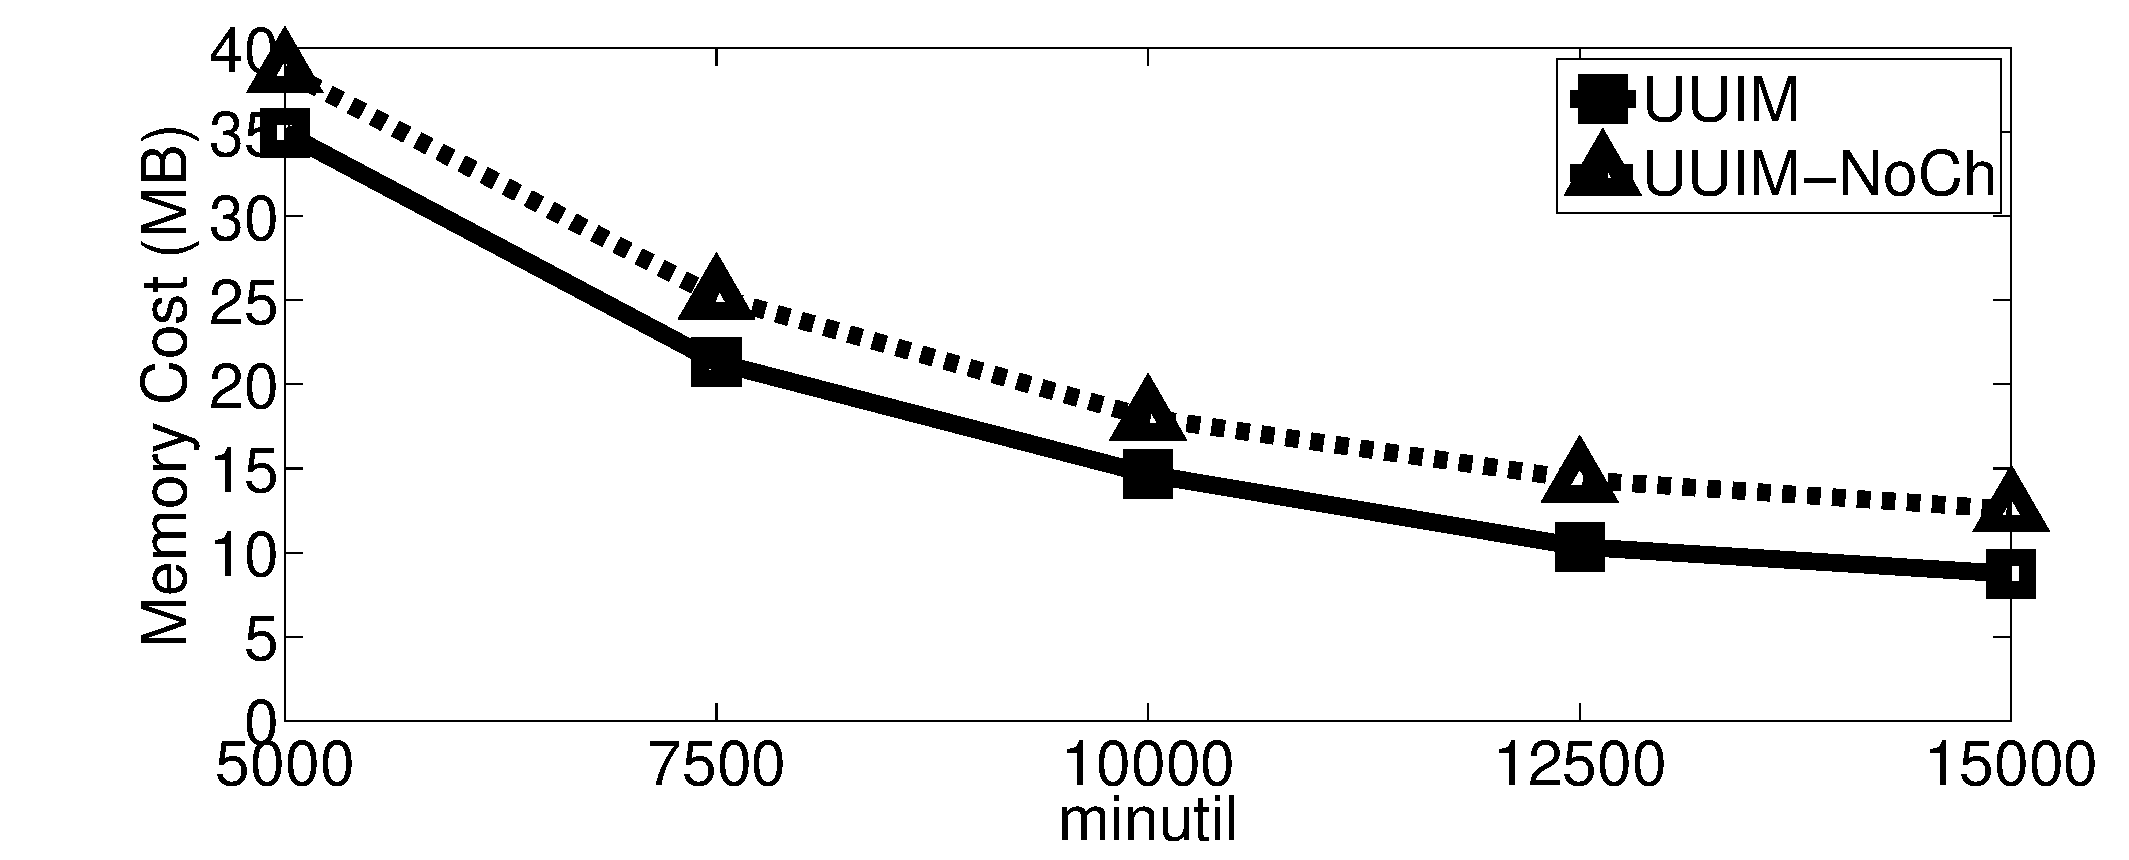
\includegraphics[width=0.99\textwidth]{7.eps}\\
  \caption{Memory Cost vs. Minimum Uility Threshold}\label{fig7}
  \vspace{-0.3cm}
\end{figure}

Fig. \ref{fig7} shows the comparison of UUIM and UUIM-NoCh on Mushroom dataset. We can see that while the utility threshold goes higher, the memory cost of these two algorithms decreases, and the difference between UUIM and UUIM-NoCh is very small, hence we can conclude that the operation of adding transaction maximum utility to header table doesn't have obvious effect.

Fig. \ref{fig8} shows the memory cost of UUIM and UUIM-NoCh in different probabilistic utility threshold. It shows that probabilistic utility threshold has almost no effect on memory cost. Besides, there is no difference between the memory cost of two algorithms.


\begin{figure}[htbp]
  \centering
  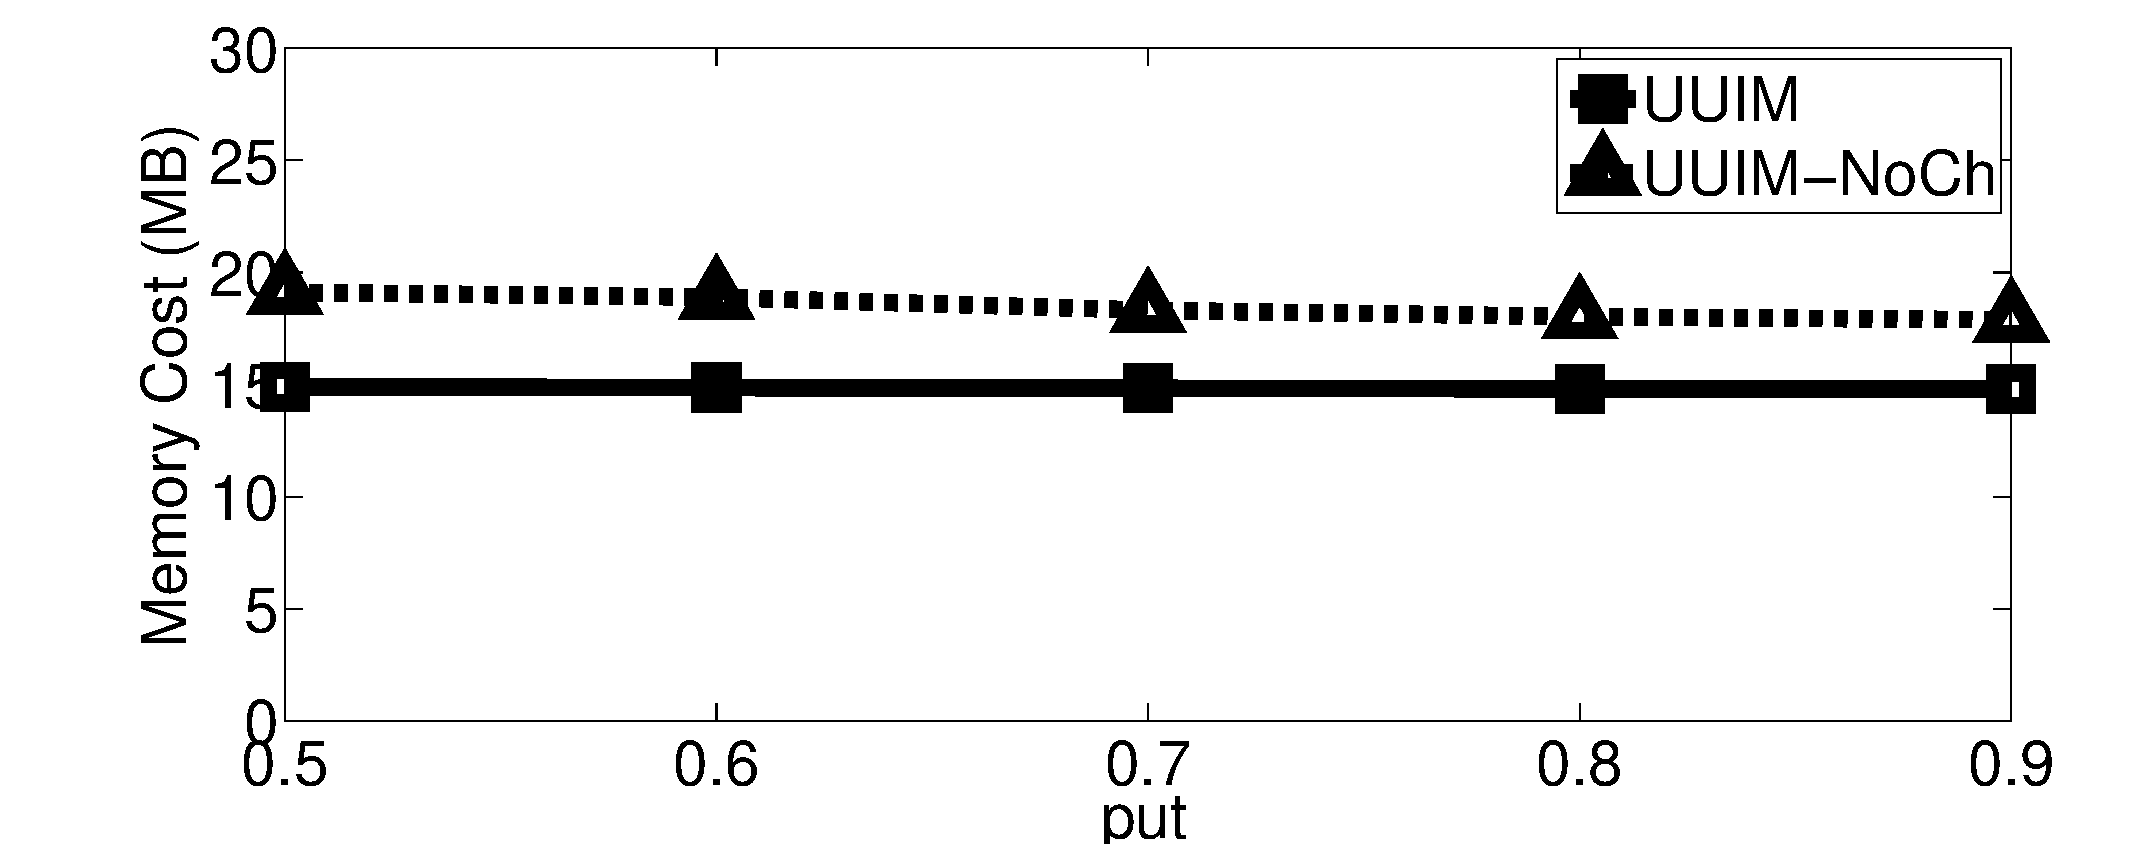
\includegraphics[width=0.99\textwidth]{8.eps}\\
  \caption{Memory Cost vs. Probabilistic Uility Threshold}\label{fig8}
  \vspace{-0.3cm}
\end{figure}

Therefore, although Chernoff bound pruning strategy needs more space, it's influence on total memory cost is small, so the strategy almost has no effect on the memory cost of the algorithm.

\subsection{Experiments conclusion}

In ��algorithm efficiency evaluation�� experiment, we can clearly see that the efficiency of UUIM algorithm is much more than UUIM-NoCh, and the difference get bigger while the utility threshold and the probabilistic utility threshold goes higher.

In ��Memory cost evaluation�� experiment, we can see that two algorithms need same memory in different utility threshold and probabilistic utility threshold. Thus the Chernoff bound pruning strategy doesn't increase the memory cost.

In summary, our UUIM algorithm is obviously better than base algorithm.

\section{Related Work}
\label{sec:related}
In this section, we review the related work in two categories, mining frequent itemsets in deterministic and uncertain data.

\subsection{Deterministic High Utility Itemset Mining}
Since Rakesh Agrawal first proposed the concept of mining frequent itemsets (or called mining large itemset) \cite{DBLP:conf/vldb/AgrawalS94}, many efficient algorithms about mining frequent itemsets have been designed, such as FP-growth \cite{DBLP:conf/sigmod/HanPY00}, Eclat \cite{DBLP:journals/tkde/Zaki00}, and so on. 

Especially, utility itemset mining, also generally called utility pattern mining, was first introduced in \cite{DBLP:conf/sdm/YaoHB04}. Although the UMining algorithm was proposed by \cite{DBLP:conf/sdm/YaoHB04}, it cannot extract the complete set of them. A transaction-weighted downward closure property was introduced in \cite{DBLP:conf/pakdd/LiuLC05}, in which a two-phase algorithm was proposed and performed faster than UMining. Moreover, IHUP \cite{DBLP:journals/tkde/AhmedTJL09} maintains the high utility patterns in an incremental
environment; since it avoids multiple scans of the database, its efficiency is far better than \cite{DBLP:conf/pakdd/LiuLC05}. Recently, UP-Growth \cite{DBLP:conf/kdd/TsengWSY10,DBLP:conf/kdd/WuSTY12} also uses a tree structure, UP-Tree, to mine high utility itemsets. Compared to IHUP, UP-Growth is more efficient, since it further reduces the number of promising patterns which cannot be pruned in IHUP.

%To solve such problem, some alternative approaches were proposed instead of mining complete frequent itemsets, such as mining frequent closed itemsets \cite{DBLP:conf/icdt/PasquierBTL99}, mining frequent maximal itemsets \cite{DBLP:conf/sigmod/Bayardo98}, mining non-derivable frequent itemsets \cite{DBLP:conf/pkdd/CaldersG02}, etc. These alternative methods can be grouped into two categories: the lossless compression-based methods and lossy compression-based methods. Among above approaches, mining frequent closed and non-derivable itemsets are lossless compression-based methods. The others belong to the lossy compression-based methods. Moreover, even though there are a lot of studies on mining frequent itemsets, all these approaches do not concern the correlated property of uncertain data.

\subsection{Uncertain Frequent Itemset Mining}
Another set of related researches with our work is the issues of mining frequent itemsets over uncertain data. Different from the certain case, the definition of a frequent itemset in uncertain data has two types of probabilistic semantics: \textit{expected support-based frequent itemset} \cite{DBLP:conf/kdd/AggarwalLWW09,DBLP:conf/pakdd/ChuiKH07} and \textit{probabilistic frequent itemset} \cite{DBLP:conf/kdd/BerneckerKRVZ09}. In the definition of the expected support-based frequent itemset, the expectation of the support of an itemset is defined as the measurement, called as the expected support of this itemset \cite{DBLP:conf/kdd/AggarwalLWW09,DBLP:conf/pakdd/ChuiK08,DBLP:conf/pakdd/ChuiKH07,DBLP:conf/pakdd/LeungMB08}. In the definition of probabilistic frequent itemset \cite{DBLP:conf/kdd/BerneckerKRVZ09,DBLP:conf/kdd/SunCCC10,DBLP:conf/cikm/WangCLC10}, the probability that an itemset appears at least the minimum support (\textit{min\_sup}) times is defined as the measurement, called as the frequent probability of an itemset. Recently, \cite{DBLP:journals/pvldb/TongCCY12} using an experimental method shows the aforementioned two definitions of uncertain frequent itemsets is actually equivalent while the uncertain databases are very large.

Although there are related researches of mining frequent itemsets over uncertain data, all of them are built over the assumption that each item has no unit profit and only appear once in each transaction. In other words, none of existing work cannot address the problem of mining probabilistic high utility itemsets over uncertain data. 


\section{Conclusion}

In this paper, we formulate a new type of problem of mining uncertain frequent itemsets, called \textit{\underline{m}ining \underline{p}robabilistic \underline{h}igh \underline{u}tility itemsets in uncertain databases} (MPHU), where each item has an unit profit and likely appears multiple times in one transaction. In order to solve the \textit{MPHU} problem, we propose a novel mining framework, called \textit{UUIM}, which not only includes an efficient mining algorithm but also contains an effective pruning technique. Extensive experiments on both real and synthetic datasets verify the effectiveness and efficiency of proposed solutions.

\bibliographystyle{splncs03}
\bibliography{cup}
\end{document}
